\chapter{Artificial Compressibility}

\modinfo{Module name}{\Idx{ArtificialCompressibility}}
%\modinfo{Module subroutines}{\Idx{CompressibilityScale}, Idx{CompressibilitySolver}}
\modinfo{Module subroutines}{\Idx{CompressibilityScale}}
\modinfo{Module authors}{Peter R�back}
\modinfo{Document authors}{Peter R�back}
\modinfo{Document created}{16.2.2002}
\modinfo{Document edited}{8.2.2006}

\section{Introduction}

When \Idx{fluid-structure interaction} (FSI) problems are 
solved with a loosely coupled
iteration strategy there is a risk of applying unphysical boundary 
conditions that lead to severe convergence problems.
The reason for this is that initially the 
fluid domain is unaware of the constraint of the structural
domain, and vice versa. If the iteration converges this 
discrepancy will be settled, but sometimes the initial 
phase is so ill posed 
that convergence is practically 
impossible to obtain~\cite{jarvinen01,formaggia00}.
 
The problem may be approached by applying the 
method of \Idx{artificial compressibility}
to the fluid-structure interaction.
Previously artificial compressibility has mainly been used as a trick 
to eliminate the pressure from the Navier-Stokes equations 
or to improve the convergence of the solution 
procedure~\cite{chorin97,rogers87,carter91}. 
Here the compressibility is defined so that it 
makes the fluid imitate the elastic response of 
the structure.

The method is best suited for cases where there is a direct
correspondence between the pressure and the volume. Inertial
forces and traction forces should be of lesser importance.
The method might, for example, boost up the modeling of
human arteries.


\section{Theory}

\subsection{Fluid-structure interaction}
The theoretical model with some results is thouroughly presented in

We look at the time-dependent fluid-structure interaction
of elastic structures and incompressible fluid. 
The equations of momentum in the structural domain is
\begin{equation}
\rho\frac{\partial^2 \vec{u}}{\partial t^2} = \nabla\cdot \tau
+ \vec{f} \, \, \mbox{in} \,\, \Omega_s,
\end{equation}
where $\rho$ is the density, 
$\vec{u}$ is the displacement, $\vec{f}$ the applied 
body force and $\tau=\tau(\vec{u})$ the stress tensor 
that for elastic materials may 
be locally linearized with $\vec{u}$.
For the fluid fluid domain the equation is 
\begin{equation}
  \rho\left( \frac{\partial\vec{v}}{\partial t} 
+ \vec{v}\cdot\nabla\vec{v} \right) 
        =  \nabla\cdot\sigma+ \vec{f}\, \, \mbox{in} \, \, \Omega_f,
\end{equation}
where $\vec{v}$ the fluid velocity and
$\sigma$ the stress tensor.
For Newtonian incompressible fluids the stress is
\begin{equation}
  \sigma = 2 \mu \varepsilon (\vec{v}) - pI,
\end{equation}
where $\mu$ is the viscosity, $\varepsilon(\vec{v})$ the 
strain rate tensor and $p$ the pressure.
In addition the fluid has to follow the equation of continuity
that for incompressible fluid simplifies to 
\begin{equation}
\nabla\cdot \vec{v} = 0 \, \, \mbox{in} \, \, \Omega_f.
\end{equation}
For later use we, however, recall the general form 
of the \Idx{continuity equation},
\begin{equation}
\frac{\partial\rho}{\partial t}+\nabla\cdot (\rho \vec{v}) = 0 \, \, \mbox{in} \, \, \Omega_f.
\label{eqcontgen}
\end{equation}

The fluid-structure interface, $\Gamma_{fs}$, must meet 
two different boundary conditions.
At the interface the fluid and structure 
velocity should be the same,
\begin{equation}
\vec{v}(\vec{r},t) = \dot{\vec{u}}(\vec{r},t), \,\,\, \vec{r} \in \Gamma_{fs}.
\label{cond2}
\end{equation}
On the other hand, 
the surface force acting on the structure, $\vec{g}_s$, 
should be opposite to the force acting on the 
fluid, $\vec{g}_f$, thus
\begin{equation}
\vec{g}_s(\vec{r},t)= -\vec{g}_f(\vec{r},t), \,\,\, \vec{r} \in \Gamma_{fs}.
\label{cond1}
\end{equation}

A widely used iteration scheme in FSI is the following:
First, assume a constant geometry and solve the Navier-Stokes
equation for the fluid domain with fixed boundary conditions
for the velocity. Then calculate the surface forces acting on the 
structure. Using these forces solve the structural problem.
Using the resulting displacement velocities as fixed 
boundary conditions resolve the fluid domain. Continue the 
procedure until the solution has converged. 

The above described iteration usually works quite well.
However, in some cases the boundary conditions~(\ref{cond2})
and~(\ref{cond1}) lead to problems. 
The elasticity solver is not aware of 
the divergence free constraint of the velocity field.
Therefore the suggested
displacement velocities used as boundary conditions
may well be such that there is no solution for the
continuity equation. A proper coupling method 
makes the solution possible even if the velocity boundary 
conditions aren't exactly correct.
Further, if the Navier-Stokes equation is 
solved without taking into account the elasticity of
the walls, the forces in equation (\ref{cond1}) will be 
exaggerated. The pathological case is one where all the 
boundaries have fixed velocities. Then even an infinitely small
net flux leads to infinite pressure values. A proper  coupling method
should therefore also give realistic pressure values even with inaccurate
boundary conditions. The method of artificial compressibility 
meets both these requirements.


\subsection{Artificial compressibility}

When a surface load is applied to an elastic container
it results to a change in the 
volume. In many cases of practical interest 
the change in volume is mainly due to a pressure variation
from the equilibrium pressure
that leads to zero displacements. 
If the structural domain is described by linear equations
the change in volume $dV$ has a direct
dependence on the change in the pressure, $dP$, or
\begin{equation}
  \frac{dV}{V} = c \, dP. \label{eq_comp1}
\end{equation}
This assumption limits the use of the model in highly
nonlinear cases.

The change in the volume should be the same 
as the net volume flux into the domain.
As this cannot be guaranteed during the iteration,
some other way to enable the material conservation must be used. 
A natural choice is to let the density 
of the fluid vary so that is has the same pressure response
as the elastic walls,
\begin{equation}
  \frac{d\rho}{\rho} = c \, dP,
\end{equation}
where $c$ is the artificial compressibility.
This is interpreted locally and inserted
to the continuity equation~(\ref{eqcontgen}) while neglecting
the space derivative of the density, thus
\begin{equation}
c \, \frac{dp}{dt} + \nabla\cdot \vec{v}  = 0,
\end{equation}
where $dp$ is the local pressure change.
Here the time derivative of pressure must be understood as
an iteration trick. A more precise expression is 
\begin{equation}
\frac{c}{\Delta t} \left( p^{(m)}-p^{(m-1)}\right) + \nabla\cdot \vec{v}^{(m)}  = 0,
\end{equation}
where $m$ is the current iteration step related to fluid-structure
coupling. When the iteration converges $p^{(m)} \rightarrow p^{(m-1)}$
and therefore the modified equation is consistent with the 
original one.
The weak form of the equation for finite element method (FEM)
may easily be written, 
\begin{equation}
  \int_{\Omega_f} (\nabla \cdot \vec{v}^{(m)}) \varphi_p \, d\Omega + 
  \frac{1}{\Delta t} \int_{\Omega_f} c \left(p^{(m)} - p^{(m-1)}\right) \varphi_p \, d\Omega = 0,
\end{equation}
where $\varphi_p$ is the test function.  

The artificial compressibility may be calculated 
analytically in simple geometries. For example, 
for a thin cylinder with thickness $h$ and radius $R$
the compressibility is $c = 2R/Eh$~\cite{riemslagh00}, where $E$ is the 
Young's modulus, and correspondingly for a sphere $c = 3R/Eh$.

In most practical cases the elastic response of the
structure cannot be calculated analytically.
Then the compressibility may also be computed from 
equation (\ref{eq_comp1}) by applying a pressure change
$dP$ to the system, 
\begin{equation}
  c = \frac{1}{V}\frac{dV}{dP}.
\end{equation}
The change in volume may be calculated  by 
comparing it to initial volume, thus
 \begin{equation}
  c = \frac{V-V_0}{V_0}\frac{1}{dP}.
  \label{eq:v0}
\end{equation}

For small deformations $ds=\vec{u}\cdot\vec{n}$,
where $\vec{n}$ is the surface normal.
Therefore we may use an alternative form 
convenient for numerical computations, 
\begin{equation}
  c = \frac{\int_{\Gamma_{fs}} (\vec{u}\cdot\vec{n}) \, dA}{\int_{\Omega_f} dV} 
	\frac{\int_{\Gamma_{fs}} dA}{\int_{\Gamma_{fs}} dp \,dA}.
\end{equation}
This way $c$ has a constant value over the domain. 


\subsection{Scaling artificial compressibility}

If the artificial compressibility distribution is a priori defined 
we may use the above equations to scale the compressibility 
appropriately. For example, the 
compressibility could be given only within a limited distance from the elastic wall.
and the functional behavior of $c(\vec{r})$ would be
user defined. Computing compressibility becomes then just 
a matter of scaling,
\begin{equation}
  c(\vec{r}) = c_0(\vec{r}) \underbrace{
\frac{\int_{\Gamma_{fs}} (\vec{u}\cdot\vec{n}) \, dA}{\int_{\Omega_f} c_0(\vec{r}) dV} 
	\frac{\int_{\Gamma_{fs}} dA}{\int_{\Gamma_{fs}} dp \,dA}}_{\mbox{scaling factor}}.
\end{equation}

A suitable test load for computing compressibility is 
the current pressure load on the structure. 
However, for the first step the compressibility must
be predefined. It is safer to over-estimate it since that leads to
too small a pressure increase. Too large a pressure increase might ruin
the solution of the elasticity solver and by that also the 
computational mesh used by the flow solver would be corrupted.
Therefore some sort of exaggeration factor exceeding unity
might be used to ensure convergence.


\subsection{Elementwise artificial compressibility}

If the displacement field is extended smoothly throughout the whole 
geometry it may be possible to define the artificial compressibility 
separately for each element or node. This is particularly usefull for geometries 
where the elastic response changes significantly. 
The equation is now similar to (\ref{eq:v0}),
\begin{equation}
  c = \frac{V^e-V^e_0}{V^e_0}\frac{1}{dP},
\end{equation}
where the superscript $e$ refers to the volume of an element. 
This may also be solved using finite element strategies
to get nodal values for $c$.


\section{Keywords} 

\subsection*{Keywords of FlowSolve}

\sifbegin
\sifitem{Material}{mat id}
In the material section the compressibility model
and the initial artificial compressibility field is given.
\sifbegin
\sifitem{Compressibility Model}{String [Artificial Compressible]}
Set the meterial model of the fluid. 
\sifitem{Artificial Compressibility}{Real}
The initial value of artificial compressibility. This may also be a distributed 
function that is then scaled by the solver.
\sifend
\sifend


\subsection*{Keywords of solver CompressibilityScale}

If the artificial compressibility is tuned so that it best
imitates the elastic response, a additional solver must be 
used to rescale the above mentioned compressibility.
The solver computes the total compressibility and the force acting
on the surface. The compressibility is integrated over all volumes
that are solved with the navier-stokes equation.

\sifbegin
\sifitemnt{Solver}{solver id}
\sifbegin
\sifitem{Equation}{String CompressibilityScale}
The name of the solver.
\sifitem{Procedure}{File "ArtificialCompressibility" \\ "CompressibilityScale"}
The subroutine in the dynamically linked file.
\sifitem{Steady State Convergence Tolerance}{Real}
How much the relative value of the compressibility may change between 
iterations, $\mbox{abs}(c_i-c_{i-1})/c_i < \varepsilon$.
\sifitem{Nonlinear System Relaxation Factor}{Real}
Relaxation scheme 
$c'_i=\lambda c_i + (1-\lambda)c_{i-1}$
for the compressibility.
By dafault is $\lambda=1$. 
\sifend

\sifitemnt{Boundary Condition}{bc id}
\sifbegin
\sifitem{Force BC}{Logical}
The elastic response is calculated over the surface(s) which has this definition
as {\tt True}.
\sifend
\sifend


\subsection*{Keywords of solver CompressibilitySolver}

When the compressibility is solved elementwise using this solver there has to usually 
be a isobaric steady-state test phase where the compressibility is defined. 
For this solver all the normal \texttt{Linear System} keywords also apply.

\sifbegin
\sifitemnt{Solver}{solver id}
\sifbegin
\sifitemnt{Equation}{String CompressibilitySolver}
\sifitemnt{Procedure}{File "ArtificialCompressibility" \\ "CompressibilitySolver"}
\sifitem{Variable}{String ac}
The name of the artificial compressibility field variable.
\sifitem{Displacement Variable Name}{String "Mesh Update"}
The name of the displacement field variable that is used to compute the 
the volume change.
\sifitem{Displaced Shape}{Logical True}
Flag that defines whether the current shape is the displaced or original
shape.
\sifitem{Reference Pressure}{Real}
The value of pressure used for the test loading.
\sifend
The computed field should then be given as the value 
in the material section.
\sifitemnt{Material}{mat id}
\sifbegin
\sifitem{Artificial Compressibility}{Equals ac}
The initial value of artificial compressibility given by the solver.
\sifend
\sifend


\subsection{Examples}

The examples show a 2D square and a 3D cube being gradually filled. 
The fluid comes in from one wall and the opposing elastic wall 
makes room for the fluid so that the continuity equation is satisfied.
Here the value of artificial compressibility is scaled every timestep to
account for the nonlinear elasticity.

\begin{figure}[tbhp]
\begin{center}
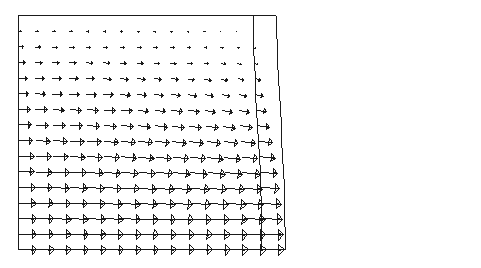
\includegraphics[width=0.45\textwidth]{fill2.png}
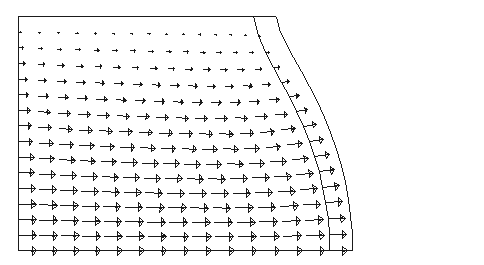
\includegraphics[width=0.45\textwidth]{fill20.png}
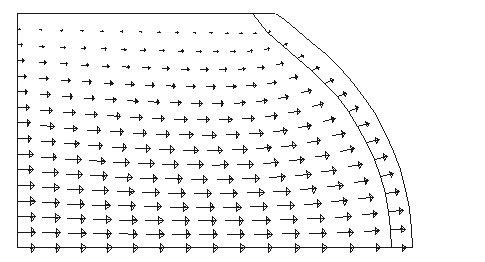
\includegraphics[width=0.45\textwidth]{fill40.png}
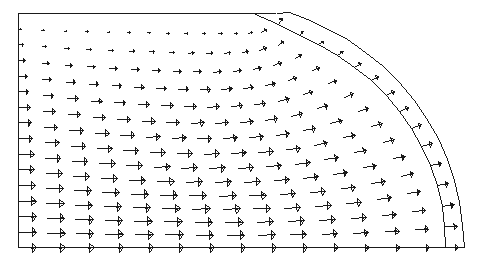
\includegraphics[width=0.45\textwidth]{fill60.png}
\end{center}
\caption{Snapshots of an elastic square being gradually filled by incompressible fluid.}
\end{figure}

\begin{figure}[tbhp]
\begin{center}
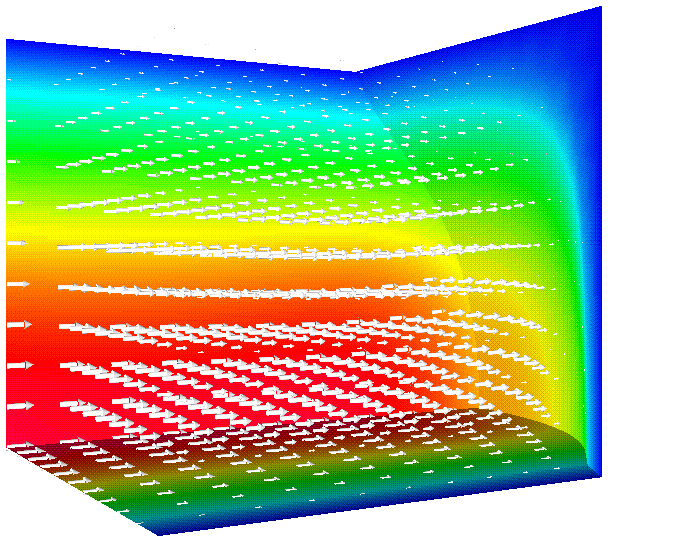
\includegraphics[width=0.45\textwidth]{box3d20.png}
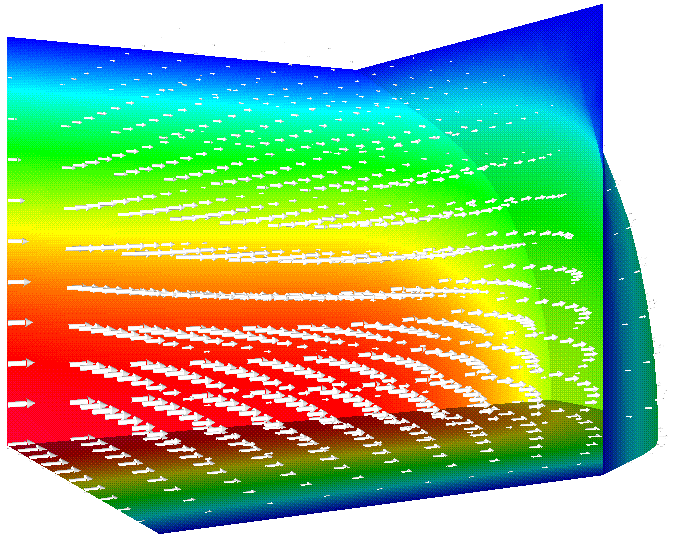
\includegraphics[width=0.45\textwidth]{box3d39.png}
\caption{Snapshots of an elastic cube being gradually filled by incompressible fluid.}
\end{center}
\end{figure}


\bibliography{elmerbib}
\bibliographystyle{plain}
